% ===============================================================
%  Relatório Técnico: Sistema Pericial de Apoio à Condução
%  PPROGIA
%
%  Compilação:  ./build.sh
%          ou:  latexmk -pdf relatorio.tex
%          ou:  pdflatex relatorio && bibtex relatorio && pdflatex relatorio x2
% ===============================================================

% 11pt é a base da classe; o tamanho real do texto (10.5pt) é definido em
% preambulo.tex, secção COMPACTAÇÃO LIGEIRA, com o scrextend.
\documentclass[11pt,a4paper,oneside]{report}

% ---------------------------------------------------------------
% metadados.tex
% Editar APENAS este ficheiro para personalizar a capa do relatório.
% ---------------------------------------------------------------

\newcommand{\instituicao}{Instituto Superior de Engenharia do Porto}
\newcommand{\instituicaosigla}{ISEP}
\newcommand{\curso}{Mestrado em Engenharia de Inteligência Artificial}
\newcommand{\cursosigla}{MEIA}
\newcommand{\uc}{Paradigmas de Programação em Inteligência Artificial}
\newcommand{\ucsigla}{PPROGIA}
\newcommand{\anoletivo}{2026/2027}
\newcommand{\semestre}{1.\textordmasculine{} Semestre}

\newcommand{\tituloprincipal}{Sistema Pericial de Apoio à Condução}
% Só para a capa: o mesmo título, com a quebra de linha escolhida (o cabeçalho e os
% metadados do PDF usam \tituloprincipal, sem quebra).
\newcommand{\titulocapa}{Sistema Pericial de\\Apoio à Condução}
\newcommand{\subtitulo}{Relatório Técnico}
\newcommand{\descricao}{Motor de inferência, base de conhecimento,\\
meta-conhecimento e explicação em Prolog}

% ---------------------------------------------------------------
% Autoria
%
% Para acrescentar, remover ou reordenar autores, basta editar a lista
% abaixo: uma linha \autor{nome}{email} por elemento. A capa
% acompanha automaticamente, seja qual for o número de autores.
% ---------------------------------------------------------------
\providecommand{\autor}[2]{}

\newcommand{\listaautores}{%
  \autor{Ana Salomé Ferreira Teixeira}{1210803@isep.ipp.pt}%
  \autor{Diogo Miguel Gonçalves Ribeiro}{1260429@isep.ipp.pt}%
  \autor{João Gabriel Domingos de Azevedo}{1211519@isep.ipp.pt}%
  \autor{Pedro Nuno Verde Cerqueira}{1260443@isep.ipp.pt}%
  \autor{Rúben Alexandre Abreu Freitas}{1231267@isep.ipp.pt}%
  \autor{Rúben Carlos Zamith Ribeiro}{1161532@isep.ipp.pt}%
}

% Nomes usados nos metadados do PDF (propriedades do ficheiro).
\newcommand{\autoresmeta}{%
  Ana Salomé Ferreira Teixeira;
  Diogo Miguel Gonçalves Ribeiro;
  João Gabriel Domingos de Azevedo;
  Pedro Nuno Verde Cerqueira;
  Rúben Alexandre Abreu Freitas;
  Rúben Carlos Zamith Ribeiro%
}

% ---------------------------------------------------------------
% Docência
%
% Mesma mecânica da autoria: uma linha \docente{nome}{email} por
% elemento.
% ---------------------------------------------------------------
\providecommand{\docente}[2]{}

\newcommand{\listadocentes}{%
  \docente{António Constantino Lopes Martins}{}%
  \docente{José Antonio Reis Tavares}{}%
  \docente{Jorge Alexandre Novo Meira}{}%
}

\newcommand{\datarelatorio}{25 de outubro de 2026}

% ---------------------------------------------------------------
% preambulo.tex — pacotes, estilos e ambientes
% ---------------------------------------------------------------

\usepackage[T1]{fontenc}
\usepackage[utf8]{inputenc}
\usepackage[portuguese]{babel}
\usepackage{lmodern}
% A bibliografia chama-se «Referências», como na versão Word do relatório.
\addto\captionsportuguese{\renewcommand{\bibname}{Referências}}
\usepackage{microtype}

\usepackage[a4paper,margin=2.6cm,headheight=15pt]{geometry}
\usepackage{graphicx}
\usepackage{booktabs}
\usepackage{longtable}
\usepackage{array}
\usepackage{tabularx}
\usepackage{multirow}
\usepackage{amsmath}
\usepackage{amssymb}
\usepackage{enumitem}
\usepackage[table]{xcolor}
\usepackage{fancyhdr}
\usepackage{titlesec}
\usepackage{caption}
\usepackage{float}
\usepackage{listings}
% Bibliografia no índice, com a página e a ligação corretas (no início da
% bibliografia), sem acrescentar o próprio índice nem as listas.
\usepackage[nottoc,notlof,notlot]{tocbibind}
\usepackage{csquotes}
% Aspas: \enquote{texto} produz “texto” (aspas duplas tipográficas).
\setquotestyle{english}
% O babel-portuguese torna " um atalho que «come» o carácter seguinte;
% desativa-se, para que aspas escritas diretamente não estraguem o texto.
\AtBeginDocument{\shorthandoff{"}}
\usepackage{icomma}        % vírgula decimal em modo matemático: $1,5$
\usepackage[most]{tcolorbox}
\usetikzlibrary{positioning}  % diagramas TikZ (o tcolorbox já carrega o tikz)

% --- Paleta ----------------------------------------------------
\definecolor{corEscura}{HTML}{1F3A5F}
\definecolor{corDestaque}{HTML}{AD451D}  % terracota do logo do MEIA
\definecolor{corSucesso}{HTML}{0B6E4F}   % verde: apenas marcadores PASSOU
\definecolor{corCinza}{HTML}{5A6672}
\definecolor{corFundo}{HTML}{F4F6F8}
\definecolor{corCritico}{HTML}{9B1C1C}
\definecolor{corAviso}{HTML}{B45309}

% obeyspaces/spaces: \cod{swipl -q -g main} mantém os espaços e pode quebrar neles.
\usepackage[obeyspaces,spaces]{url}
\DeclareUrlCommand\cod{\urlstyle{tt}}

\usepackage[pdfusetitle]{hyperref}
\hypersetup{
  colorlinks=true,
  linkcolor=corEscura,
  citecolor=corEscura,
  urlcolor=corDestaque,
  linktoc=all
}

% O cleveref não traz nomes em português; definem-se aqui.
\usepackage[capitalise,noabbrev,nameinlink]{cleveref}
\crefname{chapter}{Capítulo}{Capítulos}
\crefname{section}{Secção}{Secções}
\crefname{subsection}{Secção}{Secções}
\crefname{appendix}{Anexo}{Anexos}
\crefname{figure}{Figura}{Figuras}
\crefname{table}{Tabela}{Tabelas}
\crefname{equation}{Equação}{Equações}
\crefname{enumi}{Item}{Itens}
\newcommand{\crefrangeconjunction}{ a }
\newcommand{\crefpairconjunction}{ e }
\newcommand{\crefmiddleconjunction}{, }
\newcommand{\creflastconjunction}{ e }
% O cleveref usa o tipo «listing» para o contador lstlisting.
\crefname{listing}{Listagem}{Listagens}

% --- Cabeçalhos e rodapés --------------------------------------
\pagestyle{fancy}
\fancyhf{}
\fancyhead[L]{\small\textcolor{corCinza}{\ucsigla{} --- \cursosigla}}
\fancyhead[R]{\small\textcolor{corCinza}{\tituloprincipal}}
\fancyfoot[C]{\thepage}
\renewcommand{\headrulewidth}{0.4pt}

\fancypagestyle{plain}{%
  \fancyhf{}%
  \fancyfoot[C]{\thepage}%
  \renewcommand{\headrulewidth}{0pt}%
}

% --- Títulos ---------------------------------------------------
\titleformat{\chapter}[hang]
  {\normalfont\huge\bfseries\color{corEscura}}
  {\thechapter\hspace{12pt}\textcolor{corCinza}{|}\hspace{12pt}}{0pt}{\huge}
\titlespacing*{\chapter}{0pt}{-10pt}{24pt}

\titleformat{\section}
  {\normalfont\large\bfseries\color{corEscura}}{\thesection}{0.8em}{}
\titleformat{\subsection}
  {\normalfont\normalsize\bfseries\color{corEscura}}{\thesubsection}{0.8em}{}

% Uma secção não começa no fundo da página: se restar pouco espaço,
% passa para a página seguinte (no máximo ~1/5 da página fica em branco).
\usepackage{needspace}
\usepackage{placeins}  % \FloatBarrier: impede uma figura de passar para a secção seguinte
\usepackage{etoolbox}
\pretocmd{\section}{\Needspace{10\baselineskip}}{}{}
\pretocmd{\subsection}{\Needspace{6\baselineskip}}{}{}

% --- Legendas --------------------------------------------------
\captionsetup{font=small,labelfont={bf,color=corEscura},skip=6pt}

% --- Listagens de código ---------------------------------------
% Drools (DRL): sintaxe próxima do Java, com as palavras-chave das regras.
% Usada apenas na comparação com a regra Prolog equivalente (language=Drools).
\lstdefinelanguage{Drools}{
  morekeywords={package,import,global,function,declare,query,rule,when,
                then,end,salience,agenda-group,activation-group,no-loop,
                lock-on-active,dialect,and,or,not,exists,forall,from,
                collect,accumulate,eval,insert,insertLogical,update,modify,
                retract,delete,new,true,false,null,this,matches,memberOf,
                contains,extends,if,else,return},
  otherkeywords={agenda-group,activation-group,no-loop,lock-on-active},
  sensitive=true,
  comment=[l]{//},
  morecomment=[n]{/*}{*/},
  string=[b]",
  morestring=[b]'
}

\lstdefinestyle{codigo}{
  basicstyle=\ttfamily\footnotesize,
  keywordstyle=\color{corEscura}\bfseries,
  commentstyle=\color{corCinza}\itshape,
  stringstyle=\color{corDestaque},
  numbers=left,
  numberstyle=\tiny\color{corCinza},
  numbersep=8pt,
  backgroundcolor=\color{corFundo},
  frame=leftline,
  framerule=1.2pt,
  rulecolor=\color{corEscura},
  framesep=8pt,
  xleftmargin=16pt,
  breaklines=true,
  breakatwhitespace=true,
  showstringspaces=false,
  columns=fullflexible,
  captionpos=b,
  language=Drools,
  literate=%
    {á}{{\'a}}1 {à}{{\`a}}1 {â}{{\^a}}1 {ã}{{\~a}}1
    {é}{{\'e}}1 {ê}{{\^e}}1 {í}{{\'i}}1
    {ó}{{\'o}}1 {ô}{{\^o}}1 {õ}{{\~o}}1
    {ú}{{\'u}}1 {ç}{{\c c}}1
    {Á}{{\'A}}1 {É}{{\'E}}1 {Í}{{\'I}}1 {Ó}{{\'O}}1 {Ú}{{\'U}}1 {Ç}{{\c C}}1
}
% Prolog (linguagem por omissão neste relatório) e JSON (pedidos ao server.pl).
% No Prolog, o apóstrofo delimita átomos ('Nome da regra'); as aspas, strings.
\lstdefinelanguage{JSON}{
  string=[b]",
  sensitive=true,
  morekeywords={true,false,null}
}
\lstset{style=codigo,language=Prolog}

\renewcommand{\lstlistingname}{Listagem}
\renewcommand{\lstlistlistingname}{Lista de Listagens}

% --- Macros auxiliares -----------------------------------------
\newcommand{\facto}[1]{\texttt{\small #1}}
\newcommand{\regra}[1]{\texttt{\small #1}}
% Identificadores de código no texto (predicados, ficheiros, classes), com
% \cod{...}: definido mais abaixo com o pacote url, que dispensa escapar os _
% de nomes como wm_support/3 e permite quebrar a linha depois de _ / . e nos
% espaços. Só ASCII dentro de \cod (para texto acentuado, usar \texttt com \_).
\newcommand{\pts}[1]{\textbf{#1}}

% Informação em falta (a obter do perito ou dos autores). Fica realçada
% para não passar despercebida para a versão final.
\newcommand{\preencher}[1]{\colorbox{corAviso!20}{\textcolor{corAviso}{\small\textbf{[#1]}}}}

% Regra em linguagem natural (SE ... ENTÃO ...), com o identificador no título.
% Uso: \begin{regranl}{R_CHUVA_01} SE ... \end{regranl}
\newtcolorbox{regranl}[1]{%
  enhanced, breakable,
  colback=corFundo, colframe=corEscura,
  boxrule=0pt, leftrule=1.2pt, arc=0pt, outer arc=0pt,
  left=8pt, right=8pt, top=4pt, bottom=4pt,
  fonttitle=\ttfamily\small\bfseries, coltitle=corEscura,
  attach title to upper, after title={\par\smallskip},
  title={REGRA \detokenize{#1}},
  fontupper=\ttfamily\small
}

\newcolumntype{L}[1]{>{\raggedright\arraybackslash}p{#1}}
\newcolumntype{C}[1]{>{\centering\arraybackslash}p{#1}}

% --- Grelha das tabelas -----------------------------------------
% V: linha vertical fina e cinzenta entre colunas, p. ex.
%    \begin{tabularx}{\textwidth}{@{}L{3cm}VX@{}}
% \linhasep: linha horizontal clara entre linhas de dados, a usar
%    depois de \\ (exceto na última linha, antes do \bottomrule).
\newcolumntype{V}{!{\color{corCinza}\vrule width 0.4pt}}
\newcommand{\linhasep}{%
  \arrayrulecolor{corCinza!45}\specialrule{0.3pt}{0pt}{0pt}%
  \arrayrulecolor{black}}
% Sem o espaço que o booktabs deixa junto às regras, para que as linhas
% verticais fiquem contínuas; o \extrarowheight compensa esse espaço.
% Aplica-se só às tabelas de conteúdo (a capa usa tabular).
\newcommand{\grelhatabelas}{%
  \setlength{\aboverulesep}{0pt}%
  \setlength{\belowrulesep}{0pt}%
  \setlength{\extrarowheight}{2pt}}
\AtBeginEnvironment{tabularx}{\grelhatabelas}
\AtBeginEnvironment{longtable}{\grelhatabelas}

% Margem extra que o TeX pode usar como ultimo recurso antes de deixar
% uma linha a transbordar. Evita \emph{overfull boxes} pontuais em
% paragrafos com termos longos em teletipo (nomes de predicados).
\setlength{\emergencystretch}{3em}

\setlist{itemsep=2pt,parsep=0pt,topsep=4pt}
\renewcommand{\arraystretch}{1.25}


\title{\tituloprincipal}
\author{\autoresmeta}
\date{\datarelatorio}

\begin{document}

% A numeração romana começa na capa (página i, sem número impresso), para que o
% leitor de PDF não a rotule como "1".
\pagenumbering{roman}
\setcounter{page}{1}

% ---------------------------------------------------------------
% capa.tex: página de rosto
% O bloco de autoria é gerado a partir de \listaautores (metadados.tex)
% e adapta-se a qualquer número de elementos.
% ---------------------------------------------------------------
\begin{titlepage}
\centering
\thispagestyle{empty}

\vspace*{0.2cm}

% --- Logotipos -------------------------------------------------
% ISEP à esquerda (marca horizontal, ~8,2:1) e MEIA à direita
% (marca vertical). O trim recorta as margens brancas do JPEG
% original; as medidas estão em bp e o ficheiro é de 72 dpi, pelo
% que correspondem a pixéis.
\noindent
\begin{minipage}[c]{0.60\textwidth}%
  \raggedright
  
\includegraphics[width=5.6cm]{logos/ISEP_logo.pdf}%
\end{minipage}%
\hfill
\begin{minipage}[c]{0.32\textwidth}%
  \raggedleft
  
\includegraphics[trim=92bp 163bp 72bp 160bp,clip,height=2.1cm]{logos/MEIA_logo.jpg}%
\end{minipage}

\vspace{0.7cm}

{\Large\scshape\textcolor{corEscura}{\instituicao}\par}
\vspace{0.3cm}
{\large\textcolor{corCinza}{\curso}\par}

\vspace{0.45cm}
\textcolor{corEscura}{\rule{\textwidth}{1.2pt}}
\vspace{0.4cm}

{\large\bfseries\textcolor{corDestaque}{\uc{} (\ucsigla)}\par}
\vspace{0.2cm}
{\normalsize\textcolor{corCinza}{\anoletivo{} \textperiodcentered{} \semestre}\par}

\vspace{0.4cm}
\textcolor{corEscura}{\rule{\textwidth}{1.2pt}}

\vspace{0.8cm}

{\Huge\bfseries\textcolor{corEscura}{\titulocapa}\par}

\vspace{0.55cm}

{\LARGE\textcolor{corCinza}{\subtitulo}\par}

\vspace{0.5cm}

{\large\textit{\descricao}\par}

\vfill

% --- Autoria ---------------------------------------------------
{\bfseries\textcolor{corEscura}{Autores}\par}
\vspace{6pt}

\begingroup
\renewcommand{\arraystretch}{1.15}
% \autorsep evita uma linha vazia no fim da tabela: fica vazio na
% primeira invocação e passa a \\ nas seguintes.
\gdef\autorsep{}%
% O \textcolor fica DENTRO do \href: de outro modo o colorlinks do
% hyperref sobrepunha-se e pintava o email com a cor das hiperligacoes.
\renewcommand{\autor}[2]{%
  \autorsep\gdef\autorsep{\\}%
  #1 & \href{mailto:#2}{\textcolor{corCinza}{\small\nolinkurl{#2}}}%
}%
\begin{tabular}{@{}l@{\hspace{1.4em}}l@{}}
\listaautores
\end{tabular}
\endgroup

\vspace{0.7cm}

{\bfseries\textcolor{corEscura}{Docência}\par}
\vspace{6pt}

\begingroup
\renewcommand{\arraystretch}{1.15}
\gdef\docentesep{}%
% Coluna única centrada; o email só aparece se não estiver vazio.
\renewcommand{\docente}[2]{%
  \docentesep\gdef\docentesep{\\}%
  #1%
  \if\relax\detokenize{#2}\relax\else
    \hspace{1.4em}\href{mailto:#2}{\textcolor{corCinza}{\small\nolinkurl{#2}}}%
  \fi
}%
\begin{tabular}{@{}c@{}}
\listadocentes
\end{tabular}
\endgroup

\vspace{0.7cm}

\textcolor{corEscura}{\rule{\textwidth}{0.6pt}}
\vspace{0.3cm}

{\normalsize\textcolor{corCinza}{\datarelatorio}\par}

\end{titlepage}

% O ambiente titlepage repõe o contador em 1 ao terminar (classe report, oneside):
% a capa é a página i, o Resumo a ii.
\setcounter{page}{2}
% COMPACTAÇÃO 2: a partir daqui (tudo menos a capa, que fica em 11pt) a letra
% passa a 10,5pt, com o \changefontsizes do scrextend (ver COMPACTAÇÃO em
% preambulo.tex). Reverter: apagar a linha seguinte.
\changefontsizes{10.5pt}

\chapter*{Resumo}
\markboth{Resumo}{Resumo}

O sistema pericial de condução decide, a cada 100\,ms, a velocidade e a faixa
de um veículo simulado. A simulação (física, sensores e mundo) está em Java. A
política de condução vive num motor de regras, e existem dois motores
intermutáveis: Drools e SWI-Prolog. Ambos implementam a interface
\cod{ExpertSystemBackend}, pelo que o \cod{SimulationEngine} não sabe qual está
ativo. O motor escolhe-se no arranque (\cod{expert.backend}) ou durante a
execução (\cod{POST /api/simulation/backend/prolog}).

A base de conhecimento Prolog replica todas as regras de decisão do Drools com
os mesmos nomes e com a saliência do Drools como precedência. Tem 120 regras:
75 com o nome exato de uma regra Drools, 43 variantes por resultado de 16 regras
Drools (por exemplo \cod{'Hold at red traffic light (emergency)'}) e 2 regras
intermédias só do Prolog. Este documento descreve o motor Prolog, a sua ligação
ao resto do sistema, o metaconhecimento dinâmico e as explicações.

Este relatório descreve um sistema pericial de apoio à condução que recebe
observações de sensores, mantém estado temporal e produz decisões explicáveis
sobre velocidade e mudança de faixa. A componente central analisada é o
\emph{backend} SWI-Prolog. O projeto não utiliza apenas o mecanismo de resolução
nativo para responder a consultas: implementa um motor próprio de regras de
produção com memória de trabalho, agenda, precedência, refração, encadeamento
para a frente e reavaliação seletiva através de um índice de dependências.

A base de conhecimento contém 120 regras declarativas que cobrem travagem de
emergência, peões, semáforos, sinais STOP, limites de velocidade, seguimento de
veículos, ultrapassagem, obstáculos, buracos, barreiras e condições
meteorológicas com lógica difusa. O motor combina estas regras com 38 tipos de
estado dinâmico. Cada ciclo da simulação envia ao processo Prolog o estado do
veículo e os eventos sensoriais em JSON. O Prolog devolve propostas, factos
derivados, verificações de segurança lateral e métricas do motor; a camada Java
arbitra as propostas em dois canais independentes, longitudinal e lateral.

A explicabilidade resulta do registo da proveniência de cada facto e de cada
proposta. O sistema responde a perguntas do tipo como foi obtida a decisão, por
que motivo venceu uma regra e por que motivo uma alternativa não foi aplicada. A
validação inclui testes unitários, testes de sequências temporais e testes de
equivalência entre Prolog e Drools. Na execução verificada para este relatório,
o \emph{build} Maven executou 598 testes sem falhas (2 ignorados).

\vspace{0.8cm}
\noindent\textbf{Palavras-chave:} sistemas periciais; Prolog; motor de
inferência; regras de produção; metaconhecimento; explicabilidade; apoio à
condução.

\clearpage


\tableofcontents
% --- LISTAS DE FIGURAS E DE TABELAS (desativadas para poupar uma página) ------
% Para as repor, tirar o "% " do início das seis linhas seguintes.
% \clearpage
% \listoffigures
% % A lista de tabelas é um \chapter*, que mudaria de página: sem o \clearpage,
% % fica na mesma página que a lista de figuras.
% \vspace{1.5cm}
% {\let\clearpage\relax\listoftables}
% --- fim das LISTAS DE FIGURAS E DE TABELAS -----------------------------------
\clearpage

\pagenumbering{arabic}
\setcounter{page}{1}

% As fontes do perito abrem a lista de referências, pela ordem em que foram
% recolhidas (unsrt numera pela ordem da primeira citação).
\nocite{cienciavitae,isepcontrato,lopes2006,uminhoteses}
% Capítulos 1 a 9 seguidos, sem mudança de página (ver CAPÍTULOS SEGUIDOS em
% preambulo.tex).
\quebracapitulofalse
\chapter{Perito}
\label{cap:perito}

O perito selecionado para apoiar este projeto foi o Professor Doutor Agostinho
Gil Teixeira Lopes, Professor Adjunto do Departamento de Engenharia Informática
do Instituto Superior de Engenharia do Porto (ISEP). A sua formação e
experiência abrangem áreas diretamente relacionadas com o projeto, nomeadamente
robótica, sistemas autónomos, visão por computador, inteligência artificial,
sensores, automação e controlo \preencher{fontes da biografia}.

Concluiu a licenciatura em Informática e Matemáticas Aplicadas em 2002, na
Universidade Portucalense, e o doutoramento em Engenharia Informática em 2006,
na Cranfield University, no Reino Unido, com especialização em automação,
controlo e robótica. Desenvolveu posteriormente atividades de investigação e
pós-doutoramento relacionadas com a automatização e o controlo de processos
industriais \preencher{fonte}.

Ao longo da sua carreira, exerceu funções de investigação e docência na
Universidade do Minho e na Universidade da Maia, integrando o ISEP em outubro de
2024. A sua atividade científica inclui investigação em robótica móvel autónoma,
visão artificial, redes neuronais, localização e navegação de robôs, bem como
orientação de projetos académicos nestas áreas \preencher{fonte}.

A sua experiência justifica a escolha como perito, uma vez que lhe permite
avaliar a representação e interpretação dos dados sensoriais, os critérios de
criticidade e as regras de tomada de decisão do sistema. O seu contributo é
particularmente relevante para validar a lógica de decisão e os mecanismos de
explicação implementados no projeto.

\chapter{Implementação do Motor de Inferência}
\label{cap:motor}

O motor de inferência é um motor de regras de produção desenvolvido em
SWI-Prolog. Em cada ciclo de 100\,ms recebe o estado do veículo e os eventos dos
sensores, dispara as regras e devolve propostas de decisão, que a arbitragem em
Java transforma numa única decisão (\cref{fig:arquitetura-motores}). As secções
seguintes descrevem as regras, a memória de trabalho e o ciclo do motor, e
comparam-no com o motor da unidade curricular.

\begin{figure}[H]
  \centering
  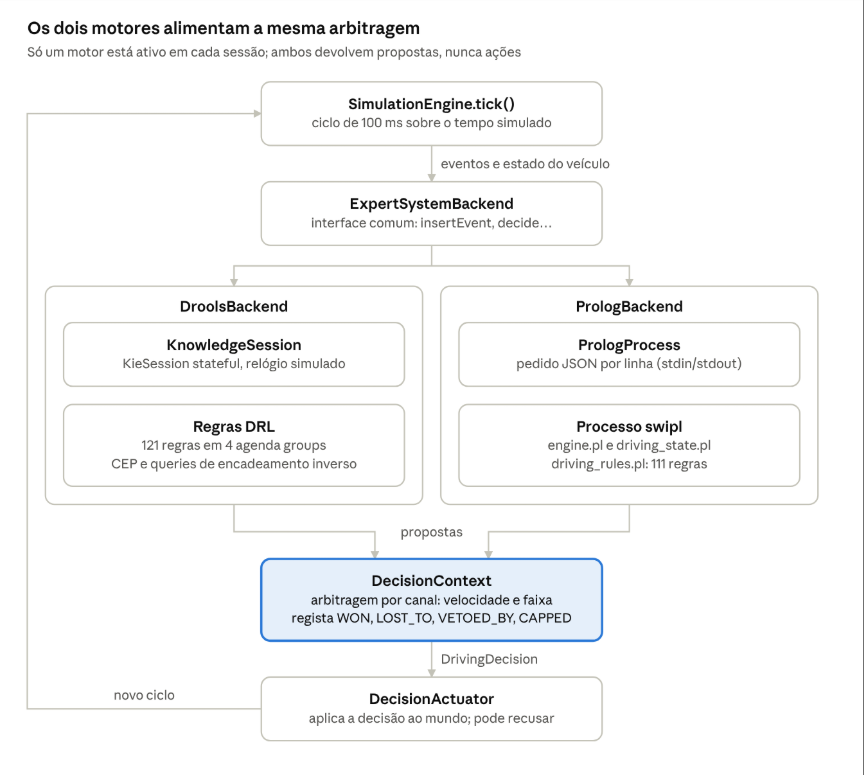
\includegraphics[width=0.78\textwidth]{figuras/arquitetura-motores.png}
  \caption{Os dois motores alimentam a mesma arbitragem: só um está ativo em
    cada sessão, e ambos devolvem propostas, nunca ações.}
  \label{fig:arquitetura-motores}
\end{figure}

\section{O motor de regras}
\label{sec:motor-regras}

As regras são dados: \texttt{rule(Id, Precedência, Condições, Ações)}. A
\cref{lst:regra-peao} mostra um exemplo.

\begin{lstlisting}[caption={Uma regra do motor Prolog (\texttt{driving\_rules.pl})},label=lst:regra-peao]
rule('Emergency stop for pedestrian extremely close',
     880,
     [ pedestrian_conflict(P),
       pedestrian(P, D),
       test(D =< 6.0) ],
     [ assert(proposal(emergency_brake, 0.0, critical, emergency_safety,
                       'Pedestrian critical distance in current path')) ]).
\end{lstlisting}

Uma condição pode ser um padrão a unificar com um facto, \cod{not(C)} (negação
por falha), \cod{test(Objetivo)} (aritmética ou um predicado auxiliar que lê os
factos através de \cod{known/1}) ou \cod{prove(Objetivo)}, provado por
encadeamento inverso (\cod{prove_goal/2}). A única ação é \cod{assert(Facto)}.
O motor faz assim encadeamento para a frente sobre os factos e encadeamento
inverso dentro das condições, por exemplo em \cod{safe_to_change_lane/1}, cujos
subobjetivos (\cod{maneuver_idle}, \cod{no_continuous_line}, \cod{side_clear},
\cod{room_to_follow}) descem até aos factos percebidos.

\begin{itemize}
  \item \textbf{Memória de trabalho:}
  \begin{itemize}
    \item \cod{wm_fact(Id, Facto)} guarda os factos do ciclo, tanto os
      percebidos como os derivados;
    \item \texttt{wm\_support(Id, Regra, Evidência)} guarda a justificação de cada
      facto derivado: a regra que o concluiu, os identificadores dos factos em
      que assentou e os padrões negados que se verificaram. Um facto sem
      suporte veio da perceção.
  \end{itemize}
  \item \textbf{Ciclo:} \cod{run_rules/0} avalia todas as regras e enche a
    agenda. Depois, até a agenda esvaziar, dispara a melhor ativação. A
    resolução de conflitos escolhe a maior precedência, depois a regra declarada
    primeiro e depois a correspondência encontrada primeiro. A refração impede
    que uma instanciação dispare duas vezes no mesmo ciclo. Os factos nunca são
    retirados dentro de um ciclo.
  \item \textbf{Estado entre ciclos:} fica em \cod{driving_state.pl}, o
    equivalente das 33 regras de perceção do Drools. Este ficheiro guarda as
    últimas leituras, a janela de TTC, o compromisso perante o semáforo, o
    cronómetro do STOP e o estado da ultrapassagem. No início de cada ciclo
    carrega tudo como factos (\cod{load_cycle_facts/0}). As regras não alteram
    estado: concluem o que mudou (por exemplo \cod{overtake_started/3}), e
    \cod{store_conclusions/0} grava-o no fim do ciclo.
\end{itemize}

\section{Comparação com o motor da unidade curricular}
\label{sec:comparacao-motor-uc}

O sistema não usa o motor da unidade curricular (\cod{sp_exp1.pl},
\cod{sp_exp2.pl}): o motor (\cod{engine.pl}) foi desenvolvido pelo grupo. O
problema exige decidir a cada 100\,ms sobre uma memória de trabalho que muda em
cada ciclo, disparar as regras pela mesma ordem que o Drools e devolver
explicações como dados ao Java, e não como texto na consola. Do motor da UC
manteve-se a ideia central: registar a justificação de cada facto quando é
concluído (\cod{justifica/3} corresponde ao nosso \cod{wm_support/3}) e
explicar a partir desse registo.

As regras do professor usam operadores e números
(\cod{regra 7 se [... e ...] entao [cria_facto(...)]}). As nossas são termos
simples, \texttt{rule(Id, Precedência, Condições, Ações)}, identificados pelo nome
da regra Drools que replicam e com uma precedência numérica. As condições do
professor são factos, \cod{nao} e \cod{avalia/1}, que compara um valor com uma
constante. As nossas acrescentam \cod{test/1}, com qualquer objetivo Prolog (por
exemplo, comparar a velocidade com o limite), e \cod{prove/1}, que prova o
objetivo por encadeamento inverso. O controlo também difere. O motor do
professor dispara uma regra assim que um facto a satisfaz. O nosso junta as
instanciações numa agenda, escolhe pela precedência e aplica refração.

A diferença principal está no metaconhecimento. No \cod{sp_exp2.pl},
\cod{facto_dispara_regras/2} indica que regras cada facto pode disparar, mas é
estático e escrito manualmente na base de conhecimento. Uma entrada em falta faz
com que a regra nunca seja tentada, sem qualquer erro. No nosso motor, o
metaconhecimento é dinâmico. \cod{ensure_index/0} deriva-o das próprias regras
quando o motor arranca, incluindo os factos lidos pelos predicados auxiliares, e
guarda-o em predicados dinâmicos (\cod{rule_reads/2}, \cod{rule_precedence/2},
\cod{rule_rank/2}). \cod{fired/2} muda a cada disparo. Nas explicações,
\cod{como/1} escreve na consola, enquanto \cod{explain/2} devolve a árvore de
derivação como termo. \cod{whynot/1} parte de um facto e desce recursivamente
pelas premissas, enquanto \cod{why_not/2} parte de uma regra e indica a condição
que a impediu de disparar. O motor do professor não tem explicação do tipo
\emph{Why}.

\chapter{Base de conhecimento}
\label{cap:base-conhecimento}

A base de conhecimento (\cod{driving_rules.pl}) é um conjunto de $\sim$120 regras de
produção sobre condução, que replicam as regras de decisão do motor Drools do
sistema.

\section{O que a base contém}
\label{sec:base-conteudo}

O objetivo é que o comportamento do veículo fique descrito nas regras, e não
espalhado pelo código de controlo. A base cobre emergências, peões, veículo da
frente e ultrapassagens, limites de velocidade, STOP, semáforos, perigos na estrada,
mudanças de via, barreiras e meteorologia. Várias regras seguem diretamente o Código da Estrada~\cite{codigoestrada}: o
Art.~13.º, n.º~3 (circular pela via mais à direita, \cref{lst:regra-direita}),
o Art.~18.º (distância ao veículo da frente), o Art.~24.º (adequar a velocidade
às condições) e os Arts.~36.º e 38.º (ultrapassar pela esquerda e regressar à
direita no fim da manobra).

As regras leem $\sim$66 tipos de facto, que se agrupam como mostra a
\cref{tab:tipos-factos}.

\begin{table}[H]
  \centering
  \caption{Tipos de facto lidos pelas regras}
  \label{tab:tipos-factos}
  \small
  \begin{tabularx}{\textwidth}{@{}L{3.0cm}V>{\raggedright\arraybackslash}XVL{4.2cm}@{}}
    \toprule
    \textbf{Tipo} & \textbf{Exemplos} & \textbf{Origem} \\
    \midrule
    Perceção & \cod{ego_speed(Kmh)}, \cod{pothole(Id, DistanceM, Severity, Lane)},
        \cod{traffic_light(Id, red|yellow|green, DistanceM)},
        \cod{lane_occupancy(Side, Occupied, FrontDistanceM)}
      & Sensores e veículo, carregados por \cod{driving_state.pl} no início do
        ciclo \\ \linhasep
    Estado anterior & \cod{overtaking/5}, \cod{light_commitment/2},
        \cod{stop_hold_started/2}, \cod{previous_decision/2}
      & Estado guardado entre ciclos (38 tipos) e a decisão anterior \\ \linhasep
    Conclusões intermédias & \cod{pedestrian_conflict(Id)},
        \cod{fuzzy_membership/3}, \cod{fuzzy_conclusion/2},
        \cod{overtake_started/3}
      & Concluídas por regras no próprio ciclo \\ \linhasep
    Propostas & \cod{proposal(Action, SpeedKmh, Risk, Priority, Reason)}
      & Concluídas por regras, arbitradas no Java \\
    \bottomrule
  \end{tabularx}
\end{table}

Além das regras e dos factos, a base tem predicados auxiliares, que leem os
factos através de \cod{known/1} (por exemplo \cod{front_vehicle_within/1}), e
subobjetivos provados por \emph{backward chaining} (\cref{sec:base-exemplos}). As
constantes numéricas, como as distâncias de paragem e o valor de cada
prioridade, não estão escritas no Prolog: chegam do Java no pedido
\cod{reset} (\cod{param/2}, \cod{priority_value/2}).

Dada a extensão recomendada para este relatório (cerca de 10 páginas), não se
inclui o diagrama completo da árvore de decisão, isto é, o fluxograma de decisão
da velocidade e da via.
Esse diagrama pode
ser consultado junto ao código-fonte do projeto (\cref{anx:mapeamento}).
O percurso que cada decisão segue nesse fluxograma pode também ser consultado
na \emph{interface} Web, através da explicação \emph{How} (\cref{sec:expl-how}).

\section{Representação e organização}
\label{sec:base-representacao}

O ficheiro \cod{driving_rules.pl} está organizado por situação (emergência,
peões, semáforos, sinal STOP, veículo da frente, ultrapassagem, perigos na
estrada, barreiras, meteorologia, velocidade, arranque e decisão base), seguido
dos subobjetivos e dos predicados auxiliares. A precedência acompanha a
urgência: as regras de emergência têm 870 a 900, as de peões 600 a 1000, as de
velocidade 205 a 310, e a decisão base é a última (60 a $-100$). Nos termos da
unidade curricular, a base tem regras de ação, que concluem uma \cod{proposal/5} (a
maioria), e regras dedutivas, que concluem factos intermédios como
\cod{pedestrian_conflict/1} ou \cod{fuzzy_conclusion/2}; a negação entra nas
condições, com \cod{not/1}, e não há regras de refutação: um facto nunca é
negado, apenas ausente. A \cref{lst:regra-limite-pl} mostra uma regra de ação.

\begin{lstlisting}[caption={Regra de excesso de velocidade em Prolog (\texttt{driving\_rules.pl})},label=lst:regra-limite-pl]
rule('Reduce speed when exceeding detected limit',
     300,
     [ ego_speed(V),
       speed_limit(Limit),
       test(V > Limit + 0.1) ],
     [ assert(proposal(reduce_speed, Limit, moderate, speed_compliance,
                       'Vehicle exceeds current legal speed limit')) ]).
\end{lstlisting}

Ou seja, se a velocidade passar o limite em vigor em mais de 0,1\,km/h,
propõe-se reduzir para o limite, com risco moderado e prioridade de cumprimento
de velocidade (20).


\section{Alguns exemplos}
\label{sec:base-exemplos}

\paragraph{Circular pela direita.} A \cref{lst:regra-direita}, uma das regras mais longas da base, aplica o Art.~13.º, n.º~3,
do Código da Estrada (circular pela via mais à direita) e usa todas as formas de
condição da \cref{sec:motor-regras}. Só propõe voltar à direita quando nada mais
exige atenção: nenhum obstáculo, buraco, barreira ou
peão em conflito, nenhum veículo a menos de 80\,m e nenhuma ultrapassagem ou
mudança de via pedida pelo condutor.

\noindent\begin{minipage}{\linewidth}
\begin{lstlisting}[caption={Uma das regras mais longas da base de conhecimento (\texttt{driving\_rules.pl})},label=lst:regra-direita]
rule('Enforce keep right road law when right lane is safe',
     460,
     [ ego_lane(Lane),                           test(Lane \== right),
       not(presentation_demo),                   lane_change_state(idle),
       prove(no_continuous_line(right)),         not(right_lane_blocked_ahead),
       time_ms(Now),                             test(Now >= 4000),
       lane_occupancy(right, false, RightFront), test(RightFront > 80.0),
       test(fresh_side_reading(right)),          not(move_off_state(true, _)),
       not(obstacle(_, _, _, _)),                not(pothole(_, _, _, _)),
       not(barrier(_, _, false, _)),             not(pedestrian_conflict(_)),
       not(test(front_vehicle_within(80.0))),    not(lane_change_request(_)),
       not(test(driver_lane_change_hold(Now))),
       not(test(current_overtaking(true, _, _, _, _))) ],
     [ assert(proposal(return_right, no_target, low, maneuver_safety,
       'Portuguese Highway Code Art. 13: Drive on the rightmost available safe lane')) ]).
\end{lstlisting}
\end{minipage}

\paragraph{Limite de velocidade.} A câmara deteta o sinal até 120\,m à frente.
O \cod{driving_state.pl} guarda-o como pendente, com a sua posição na estrada, e
carrega-o como \cod{pending_speed_limit(Kmh, SignPositionM)}. Enquanto o sinal
está à frente, \cod{'Slow down in time for the speed limit ahead'} faz o veículo
chegar a ele já ao novo limite. Quando o veículo chega ao sinal, o limite
pendente passa a \cod{speed_limit(Kmh)}, e a regra da
\cref{lst:regra-limite-pl} pode propor \cod{reduce_speed}. Os dois limites estão
separados porque, aplicado logo que o sinal era visto, o limite fazia o veículo
abrandar demasiado cedo.

\paragraph{Meteorologia.} Para a meteorologia recorre-se a lógica difusa: um
controlador de Mamdani com 8 regras, em três níveis de precedência. Duas regras
de fuzificação (360) convertem a visibilidade e a aderência de
\cod{weather/3} em graus de pertença, \cod{fuzzy_membership(Variable, Term, Degree)}. Cinco regras de inferência (355) combinam-nos, com E como mínimo e OU
como máximo, e concluem \cod{fuzzy_conclusion(Term, Degree)}
(\cref{lst:regra-difusa}). Uma regra de desfuzificação (350) agrega as
conclusões e calcula o centroide, que é a velocidade recomendada: um único teto
\cod{reduce_speed} com prioridade de perigo na estrada (40). A precedência garante
que cada nível só dispara depois do anterior.

\begin{lstlisting}[caption={Uma regra de inferência difusa (\texttt{driving\_rules.pl})},label=lst:regra-difusa]
rule('Fuzzy: poor visibility or poor grip -> very slow',
     355,
     [ fuzzy_membership(visibility, poor, V),
       fuzzy_membership(grip, poor, G),
       test(( D is max(V, G), D > 0.0 )) ],
     [ assert(fuzzy_conclusion(very_slow, D)) ]).
\end{lstlisting}

\paragraph{Mudança de via segura.} \cod{safe_to_change_lane/1} é um objetivo,
provado por \emph{backward chaining} a partir de quatro subobjetivos
(\cref{lst:safe-lane}). As regras de desvio chamam-no nas condições com
\cod{prove(safe_to_change_lane(left))}. Mudar de via é seguro se não houver
outra manobra em curso nem linha contínua, se o ângulo morto estiver livre e se
houver espaço para seguir o veículo dessa via, com 12\,m de folga
(\cod{StoppingPolicy.roomToFollow}).

\begin{lstlisting}[caption={Objetivo provado por \emph{backward chaining} (\texttt{driving\_rules.pl})},label=lst:safe-lane]
safe_to_change_lane(Side) :-
    maneuver_idle,
    no_continuous_line(Side),
    side_clear(Side),
    room_to_follow(Side).
\end{lstlisting}

\paragraph{Incerteza.} A perceção é tratada como incerta de três formas: as
leituras vagas, como a visibilidade e a aderência, passam pelo controlador
difuso; as leituras ruidosas (o radar frontal tem ruído gaussiano com desvio
padrão de 0,7\,m) só confirmam uma situação crítica quando se repetem, por
exemplo três amostras de TTC crítico numa janela de 2\,s na regra de travagem
de emergência; e as leituras que deixam de chegar são esquecidas
(\cref{sec:base-manutencao}).

\section{Acesso e manutenção}
\label{sec:base-manutencao}

Não há manutenção de verdade: cada ciclo recarrega os factos a partir do estado em
\cod{driving_state.pl}, que esquece o que deixou de ser observado
(\cod{expire_old_readings/1}). As regras só mudam editando os ficheiros.

\chapter{Meta-conhecimento}
\label{cap:metaconhecimento}

\section{Definição e finalidade}
\label{sec:meta-definicao}

Neste projeto, meta-conhecimento é o conhecimento sobre as próprias regras, e não
sobre a condução em si, usado para controlar e acelerar a inferência. Saber que
se deve reduzir a velocidade quando o limite é ultrapassado é conhecimento do
domínio, enquanto saber que a regra que o faz lê os factos \cod{ego_speed/1} e
\cod{speed_limit/1}, que tem precedência 300 e que já disparou neste ciclo é
meta-conhecimento.

Serve três fins: a resolução de conflitos, a terminação (refração) e a
eficiência (índice de dependências).

\section{Representação no motor Prolog}
\label{sec:meta-representacao}

O meta-conhecimento está em predicados dinâmicos de \cod{engine.pl}, declarados com \cod{:- dynamic}~\cite{swideclare} e separados da
memória de trabalho (\cod{wm_fact/2}, \cod{wm_support/3}, etc.), cujos
predicados têm o prefixo \cod{wm_} (\cref{tab:metaconhecimento}).

\begin{table}[H]
  \centering
  \caption{Predicados de meta-conhecimento do motor}
  \label{tab:metaconhecimento}
  \small
  % Colunas de texto em bandeira (sem justificação), para não abrir espaços.
  \begin{tabularx}{\textwidth}{@{}L{4.7cm}VL{3.9cm}V>{\raggedright\arraybackslash}X@{}}
    \toprule
    \textbf{Predicado} & \textbf{Conhecimento representado} & \textbf{Utilização} \\
    \midrule
    \cod{rule_reads(Nome/Aridade, Regra)} & Tipos de facto que cada regra lê
      & Avaliar de novo só as regras afetadas (\cod{fire/2}, \cod{rematch/1}) \\ \linhasep
    \cod{rule_precedence(Regra, P)} & Precedência de cada regra
      & Escolher a ativação seguinte (\cod{best_activation/2}) \\ \linhasep
    \cod{rule_rank(Regra, N)} & Posição da regra na base de conhecimento
      & Desempate determinístico entre regras com a mesma precedência \\ \linhasep
    \texttt{fired(Regra, Condições)} & Instanciações que já dispararam no ciclo
      & Refração (\cod{already_fired/2}) \\
    \bottomrule
  \end{tabularx}
\end{table}

Este meta-conhecimento é gerado dinamicamente, e não escrito manualmente, em dois sentidos:

\begin{enumerate}
  \item \textbf{É derivado das regras durante a execução.} Quando o motor
    arranca, \cod{ensure_index/0} calcula \cod{rule_reads/2},
    \cod{rule_precedence/2} e \cod{rule_rank/2} a partir das próprias regras
    (\cref{sec:meta-indice}) e guarda-os com \cod{assertz}~\cite{swidynamic}.
    Uma regra acrescentada ou alterada é refletida no arranque seguinte, sem
    manutenção manual, e o mesmo passo verifica que não há identificadores
    repetidos.
  \item \textbf{Muda durante a inferência.} \cod{fired/2} ganha uma entrada a
    cada disparo e é apagado no início de cada ciclo.
\end{enumerate}

\section{Índice de dependências}
\label{sec:meta-indice}

O índice (\cod{rule_reads/2}) regista, para cada regra, os tipos de facto
(\cod{Nome/Aridade}) de que depende. \cod{ensure_index/0} obtém-nos por análise
estática da regra:

\begin{itemize}
  \item cada padrão e cada padrão negado (\cod{not/1}) contam com o seu
    \cod{Nome/Aridade};
  \item em \cod{test/1} e \cod{prove/1}, contam os factos lidos com
    \cod{known/1}, no próprio objetivo e nas cláusulas dos predicados auxiliares
    que ele chama, seguidos transitivamente com \cod{clause/2}.
\end{itemize}

Com a base de conhecimento atual, o índice tem $\sim$600 entradas, para $\sim$120
regras e $\sim$66 tipos de facto. A regra
\cod{"Avoid pothole in centre lane by changing right when right is clear"}, por
exemplo, depende de nove tipos de facto, mas só três aparecem nas suas condições
(\cod{ego_lane/1}, \cod{pothole/4} e \cod{ego_speed/1}). Os outros seis, como as
marcações da estrada, a ocupação das vias e o estado da manobra, vêm dos
predicados auxiliares, sobretudo de \cod{safe_to_change_lane/1}, chamado através
de \cod{prove/1}. Um índice feito só com os padrões visíveis da regra não veria
estas dependências.

Durante a inferência, \cod{fire/2} recolhe os tipos dos factos novos que o
disparo acrescentou e, através de \cod{rule_reads/2}, avalia de novo apenas as
regras que os leem (\cod{rematch/1}). Sem o índice, todas as
regras teriam de ser avaliadas de novo depois de cada disparo.

O teste \cod{DependencyIndexBenchmarkTest} mede o efeito do índice. Corre os 14
cenários da biblioteca durante 150 ciclos cada (2\,100 ciclos) em dois processos
Prolog lado a lado, um com o índice e outro sem ele. Em todos os ciclos, as duas
execuções tomaram a mesma decisão e dispararam as mesmas regras (10\,231
disparos): o índice só muda o custo, que o próprio motor mede
(\cod{cycle_stats/3}). Com o índice, a inferência ocupa em média cerca de
1,5\,\% do ciclo de 100\,ms (\cref{tab:desempenho}). Os tempos cobrem só a
inferência, sem a comunicação JSON, e foram medidos numa única máquina (Intel
Core Ultra 7 258V, SWI-Prolog 9.2.9).

\begin{table}[H]
  \centering
  \caption{Efeito do índice de dependências (14 cenários, 2\,100 ciclos)}
  \label{tab:desempenho}
  \small
  \begin{tabularx}{\textwidth}{@{}XVC{3.1cm}VC{3.1cm}VC{1.9cm}@{}}
    \toprule
    & \textbf{Com índice} & \textbf{Sem índice} & \textbf{Redução} \\
    \midrule
    Avaliações de regras, total (por ciclo) & 258\,894 (123) & 1\,479\,720 (705)
      & 82,5\,\% \\ \linhasep
    Tempo médio por ciclo & 1,47\,ms & 6,41\,ms & 77,0\,\% \\ \linhasep
    Pior cenário (S10, chuva) & 2,64\,ms & 9,62\,ms & 72,6\,\% \\
    \bottomrule
  \end{tabularx}
\end{table}

\section{Conhecimento de controlo}
\label{sec:meta-controlo}

Entre as ativações prontas, \cod{best_activation/2} escolhe a de maior
precedência (\cod{rule_precedence/2}). Em empate, escolhe a da regra declarada
primeiro (\cod{rule_rank/2}) e, depois, a correspondência encontrada primeiro. A
precedência de cada regra é a \emph{salience} da regra Drools que ela replica,
para que os dois motores do sistema disparem pela mesma ordem. As únicas
exceções são as duas regras intermédias de peões, que só existem em Prolog
(\cref{lst:regras-ou}).

A refração usa \cod{fired/2}. Antes de uma instanciação entrar na agenda,
\cod{already_fired/2} compara as suas condições com as das instanciações que já
dispararam, por variante (\cod{=@=}), e deixa de fora as repetidas. Como os
factos nunca são retirados dentro de um ciclo, isto impede que a mesma conclusão
seja produzida repetidamente. Um limite de 5000 disparos por ciclo
(\cod{max_firings_per_cycle/1}) protege ainda contra uma base de regras mal construída,
que não pare de gerar instanciações novas, devolvendo um erro em vez de bloquear a
simulação.

\chapter{Módulo de explicação}
\label{cap:explicacao}

As explicações assentam num princípio: a justificação de cada conclusão é
registada no momento da inferência, e não reconstruída depois. É a ideia que
se manteve do motor da unidade curricular (\cref{sec:comparacao-motor-uc}),
aplicada a dois níveis. No motor Prolog, cada facto guarda
como foi obtido. Na aplicação, cada ciclo de decisão guarda as propostas das
regras e o resultado da arbitragem.

\section{O que fica registado}
\label{sec:expl-registo}

Em cada ciclo, o motor Prolog regista:

\begin{itemize}
  \item para cada facto derivado, \texttt{wm\_support(Id, Regra, Evidência)}: a
    regra que o concluiu, os factos em que assentou e os padrões negados que se
    verificaram;
  \item para cada proposta, a ação, a velocidade, o risco, a prioridade, a
    razão, a regra e a evidência. A evidência é a lista desses factos, e cada
    facto derivado indica a regra que o concluiu, por exemplo
    \cod{pedestrian_conflict(p1) (by rule '...')};
  \item os quatro subobjetivos de \cod{safe_to_change_lane/1}
    (\cod{maneuver_idle}, \cod{no_continuous_line}, \cod{side_clear},
    \cod{room_to_follow}), provados um a um nos dois lados por
    \cod{subgoal_results/2}, mesmo quando nenhuma regra propõe mudar de via;
  \item uma entrada na linha temporal por cada leitura dos sensores
    (\cod{FACT INSERTED}) e por cada regra que concluiu algo
    (\cod{RULE FIRED}).
\end{itemize}

A camada Java junta a cada proposta o seu resultado na arbitragem: venceu,
perdeu para outra, foi vetada por uma paragem obrigatória, foi limitada por um
teto de velocidade, ou foi recusada pelo atuador. Junta também um detalhe que
identifica a regra vencedora ou o motivo da recusa.

\begin{figure}[H]
  \centering
  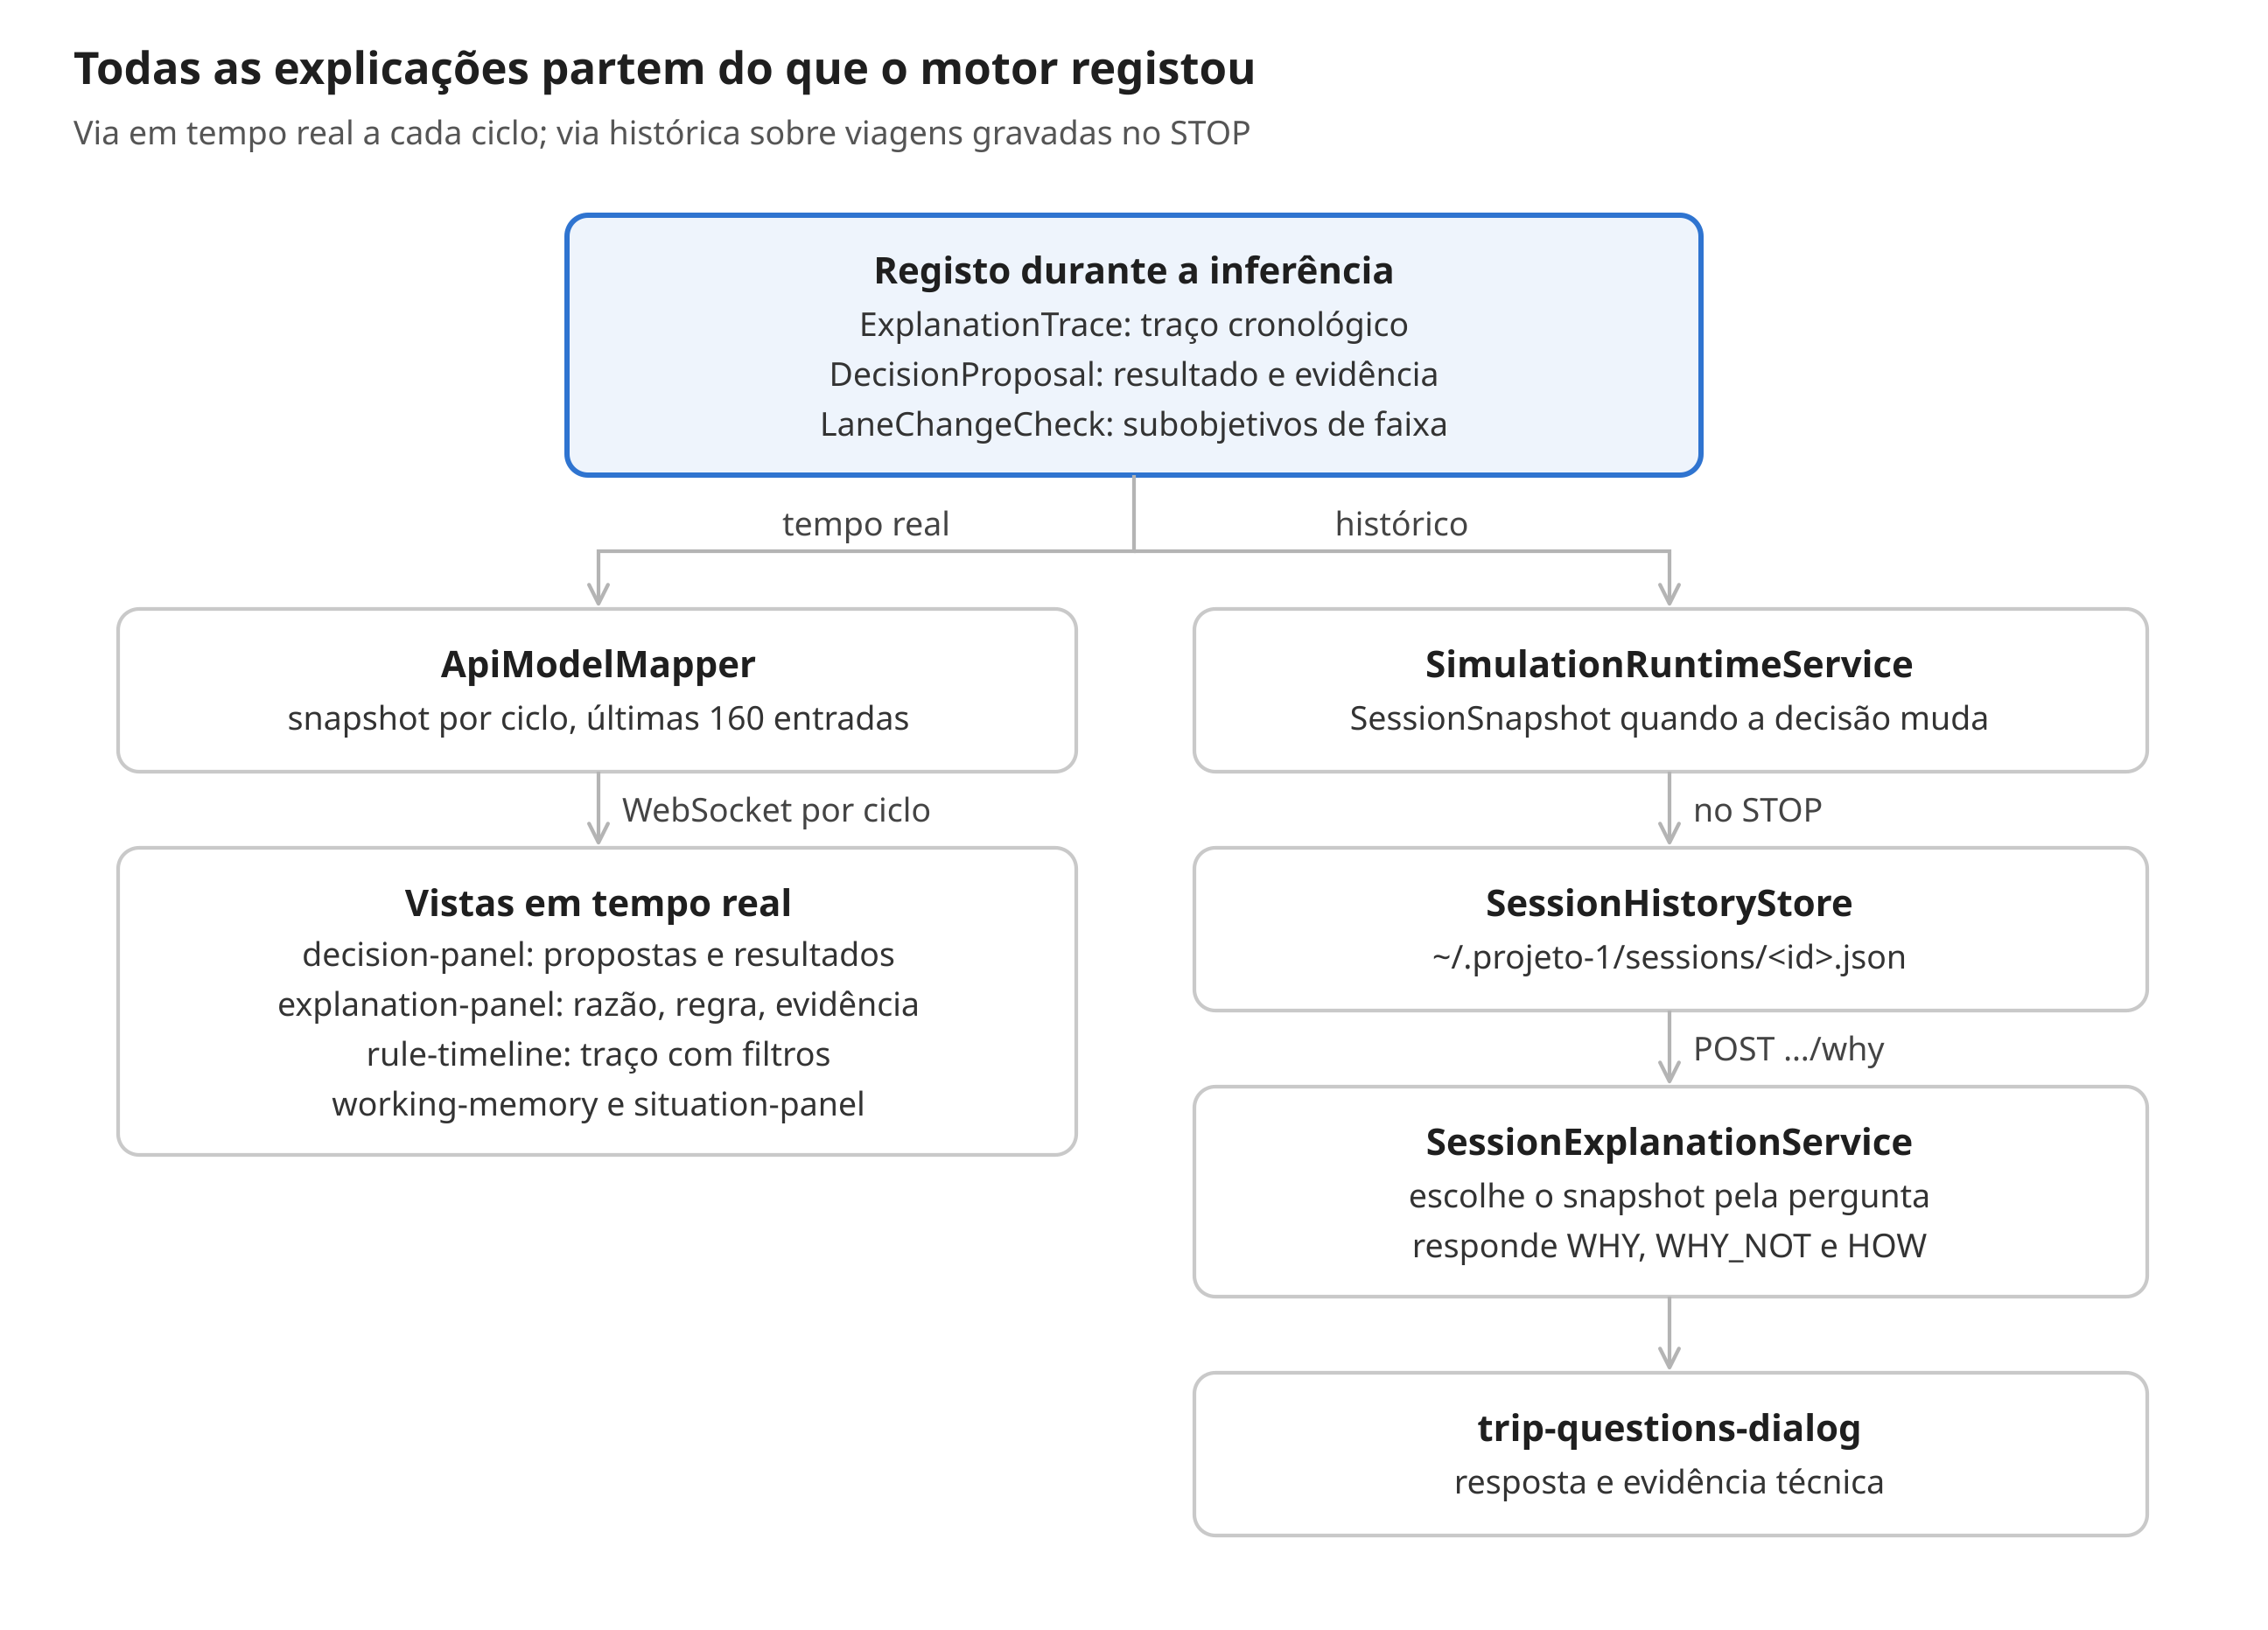
\includegraphics[width=0.70\textwidth]{figuras/explicacao-duas-vias.png}
  \caption{Percurso da informação no módulo de explicação: o percurso em tempo real, a cada ciclo, e o percurso histórico, sobre a viagem gravada ao parar.}
  \label{fig:explicacao-duas-vias}
\end{figure}

Os dois percursos da \cref{fig:explicacao-duas-vias} partem do mesmo registo. No
percurso em tempo real, o estado de cada ciclo chega à interface pelo WebSocket. O painel
de decisão mostra cada proposta com o seu resultado na arbitragem, e outros
painéis mostram a razão, a regra, a evidência, a linha temporal e a memória de
trabalho. No percurso histórico, guarda-se um registo completo do ciclo
(\cod{SessionSnapshot}) sempre que a decisão muda. Quando o utilizador carrega
no botão \enquote{STOP} da interface Web, abre-se um
diálogo em que pode percorrer as decisões registadas. Para cada uma, a interface
permite consultar os três tipos de explicação, \emph{How}, \emph{Why} e
\emph{Why not} (ver também a \cref{sec:interface}).

\paragraph{Exemplo.} Nas secções seguintes usa-se a mesma situação, executada no
motor Prolog. O veículo segue a 50\,km/h na via da direita, há um buraco na
mesma via 40\,m à frente, e a via da esquerda está livre. A regra
\cod{'Avoid pothole in right lane by changing left'} (prioridade 40) propõe
\cod{CHANGE_LANE_LEFT}, e a regra de base mantém a velocidade.

\section{How}
\label{sec:expl-how}

No motor, \cod{explain/2} percorre as justificações \cod{wm_support/3}
recursivamente e devolve a árvore de derivação como um termo. Cada facto
derivado é um nó \cod{derived(Facto, Regra, Porque)}, cada facto percebido é uma
folha \cod{perceived(Facto)}, e cada padrão negado é \texttt{absent(Padrão)}. A
\cref{lst:arvore-how} mostra a árvore da proposta do exemplo.

\begin{lstlisting}[caption={Árvore de derivação devolvida por \texttt{explain/2} para a proposta do exemplo},label=lst:arvore-how]
derived(proposal(change_lane_left, no_target, low, road_hazard,
                 'Avoiding pothole by moving into the clear left lane'),
        'Avoid pothole in right lane by changing left',
        [ perceived(ego_lane(right)),       perceived(pothole(p1,40,high,right)),
          perceived(ego_speed(50)),         perceived(lane_change_state(idle)),
          perceived(right_marking(dashed)), perceived(lane_occupancy(left,false,inf)) ])
\end{lstlisting}

A árvore tem seis factos, embora as condições da regra só nomeiem três
(\cod{ego_lane}, \cod{pothole} e \cod{ego_speed}). Os outros três vêm da prova de
\cod{safe_to_change_lane(left)}, feita por \emph{backward chaining}
(\cod{prove/1}): a prova regista os factos que lê com \cod{known/1}, e estes
passam a fazer parte da evidência. Quando a decisão depende de conclusões
intermédias, como \cod{pedestrian_conflict/1}, a árvore desce por elas.

Para obter esta árvore, optou-se por não usar o rastreio do SWI-Prolog
(\cod{trace/0}). O rastreio mostra a resolução feita pelo próprio interpretador,
com as chamadas, saídas, retrocessos e falhas de cada predicado, incluindo os do
motor (\cod{findall/3}, \cod{msort/2}), e não as regras de condução que
dispararam nem os factos em que assentaram. Além disso, é interativo e obriga
a executar em modo de depuração, mais lento. Como o motor trata as
próprias regras como dados, é ele que regista, no momento de cada disparo, a
regra e a evidência (\cod{wm_support/3}), e é desse registo que \cod{explain/2}
constrói a árvore.

Na aplicação, o \emph{How} mostra o caminho que o ciclo escolhido percorreu no
fluxograma de decisão da velocidade e no da via. Cada pergunta do fluxograma
segue o ramo \enquote{sim} quando uma das regras que lhe respondem fez uma
proposta nesse ciclo, e o caminho termina onde a arbitragem fixou a decisão.

\section{Why}
\label{sec:expl-why}

Nos materiais da unidade curricular, o \emph{Why} é o do MYCIN: quando o motor
pergunta um facto ao utilizador, este pode perguntar porquê, e o motor mostra a
regra que está a tentar provar (o \cod{sp_exp2.pl} não o
implementa). Este
sistema não faz perguntas ao utilizador. Todos os factos vêm dos sensores e do
estado do veículo, dez vezes por segundo, um ritmo a que nenhum condutor
conseguiria responder. Por isso, aqui, o \emph{Why} justifica uma decisão já
tomada: responde porque é que o veículo fez o que fez. Para cada canal, a
aplicação junta a regra que decidiu, a sua razão, a evidência e o resultado da
arbitragem, bem como as outras propostas que também foram consideradas. No canal
da via, uma mudança de via inclui ainda os subobjetivos de segurança desse
lado. No exemplo, o veículo muda para a esquerda porque
\cod{'Avoid pothole in right lane by changing left'} se verificou, com a razão
\enquote{Avoiding pothole by moving into the clear left lane}. A evidência são
os seis factos acima, e os quatro subobjetivos de
\cod{safe_to_change_lane(left)} verificaram-se. A velocidade mantém-se porque
nenhuma regra encontrou motivo para acelerar ou abrandar.

\section{Why not}
\label{sec:expl-whynot}

O \emph{Why not} responde porque é que o veículo não fez outra coisa. Na
interface, o utilizador pergunta por uma alternativa, por exemplo
\enquote{porque não abrandou para o buraco?}, e a resposta vem de dois
mecanismos. Um terceiro, no motor, desce até à condição exata de uma regra:

\begin{itemize}
  \item \textbf{Uma alternativa não escolhida.} Para cada alternativa que o
    ciclo não seguiu, na velocidade ou na via, a aplicação explica porquê, a
    partir do registo do ciclo. Ou foi proposta mas perdeu na arbitragem (e a resposta diz
    para que regra, e por que princípio), ou nunca foi proposta porque as suas
    condições não se verificaram, ou não se aplica naquele estado, ou o ciclo
    não registou o suficiente. No último caso, a resposta di-lo em vez de
    adivinhar. No exemplo, \enquote{porque não abrandou?} tem como resposta que
    nenhuma regra encontrou uma condição que exigisse abrandar, e
    \enquote{porque não mudou para a direita?} não se aplica, porque o veículo
    já está na via mais à direita.
  \item \textbf{Uma mudança de via recusada.} Os subobjetivos de
    \cod{safe_to_change_lane/1} registados em cada ciclo dizem qual deles
    falhou. Em vez de uma mensagem genérica como \enquote{mudança impossível}, a
    explicação indica a causa: outra manobra em curso, linha contínua, ângulo
    morto ocupado, ou falta de distância para seguir o veículo da outra via.
  \item \textbf{Uma regra que não disparou.} No motor, \cod{why_not/2} procura,
    entre todas as correspondências parciais das condições da regra, da esquerda
    para a direita, a que avançou mais. Devolve a condição onde parou, com as
    ligações dessa correspondência, seguida das condições posteriores que também
    falham. Chega-se a ele pelo pedido \cod{whynot} do \cod{server.pl}. No
    exemplo, para a regra que abranda perante um buraco, aponta a condição
    negada que falhou: o buraco ainda pode ser contornado (\cref{lst:whynot}).
\end{itemize}

\begin{lstlisting}[language=JSON,caption={Pedido \texttt{whynot} e resposta do \texttt{server.pl} no exemplo},label=lst:whynot]
{"cmd":"whynot", "rule":"Pothole ahead reduce speed"}
{"ok":true, "rule":"Pothole ahead reduce speed",
 "failedConditions":["not(test(pothole_avoidable_now(50,40)))"]}
\end{lstlisting}

% Capítulo resultante da fusão dos antigos capítulos "Integração do motor Prolog
% com o componente Java" e "Interface gráfica e arquitetura Web"; depois retiraram-se duas repetições.
% "do~sistema": o espaço inquebrável faz o título passar à linha depois de
% "arquitetura", com "do sistema" alinhado sob o texto do título.
\chapter{Notas adicionais sobre a arquitetura do~sistema}
\label{cap:arquitetura}

\section{Integração do motor Prolog com o componente Java}
\label{sec:integracao}

\cod{ExpertSystemBackend} define o ciclo comum aos motores: avançar o relógio,
iniciar o ciclo, inserir eventos, atualizar o veículo, decidir e expor a memória
e a explicação. \cod{PrologBackend} implementa esse contrato e permite trocar o
motor sem modificar o \cod{SimulationEngine}.

\paragraph{Comunicação.} O motor corre num processo \cod{swipl} persistente,
gerido pela classe \cod{PrologProcess}. O Java copia os ficheiros Prolog para
uma pasta de trabalho e arranca o processo com
\cod{swipl -q -g main -t halt server.pl}, que executa \cod{main/0} em \cod{server.pl}
e carrega os outros três ficheiros Prolog. Os dois lados trocam mensagens JSON
por \cod{stdin} e \cod{stdout}: um pedido por linha, e exatamente uma resposta
por linha, mesmo quando o pedido falhe. O processo é mantido vivo durante toda a
sessão: lançá-lo custa 150 a 250\,ms, incompatível com um ciclo de 100\,ms, e o
lado Prolog guarda estado entre ciclos. O \cod{server.pl} aceita quatro pedidos:
\cod{tick} (o ciclo de decisão), \cod{reset}, \cod{whynot} (\cref{sec:expl-whynot})
e \cod{dependencyIndex} (liga ou desliga o índice, só para o \emph{benchmark} da
\cref{sec:meta-indice}).

\paragraph{Pedidos e respostas.} Durante o ciclo, o \cod{PrologBackend} acumula
os eventos dos sensores. Preenche também um \cod{VehicleInput} com o estado do
veículo (velocidade, posição, via, manobra em curso, marcações e segurança das
vias adjacentes). Tudo segue num único pedido \cod{tick}, com
a decisão anterior (ação, regra e prioridade). A resposta traz as propostas
(ação, velocidade, risco, prioridade, razão, regra e evidência), os factos do
ciclo, o limite de velocidade em vigor, os subobjetivos da segurança de mudança de
via nos dois lados e as métricas do motor.

\paragraph{Arbitragem e aplicação.} O Java não decide nada por si: entrega as
propostas ao \cod{DecisionContext}. A
arbitragem trata em separado a velocidade e a via.

\begin{itemize}
  \item Na velocidade, as emergências e as paragens obrigatórias (prioridade 60
    ou mais) sobrepõem-se a tudo. Entre elas vence a mais prioritária e, em
    empate, a mais lenta. Abaixo disso, cada teto de velocidade que se verifica
    limita a velocidade de base, e decide o mais baixo, se ficar abaixo dessa
    base.
  \item Na via, vence a maior prioridade. Em empate, regressar à direita vence
    mudar de via.
  \item Uma mudança de via só é vetada quando uma paragem de prioridade
    superior está de facto a travar o veículo.
  \item Sem propostas, o veículo mantém a velocidade e a via.
\end{itemize}

O \cod{DecisionActuator} aplica a decisão ao veículo. Pode recusar uma mudança de
via que não consiga executar, e essa recusa fica registada. O ciclo, com o
resultado de cada proposta, é então guardado para o módulo de explicação
(\cref{sec:expl-registo}).

\section{Interface gráfica e arquitetura Web}
\label{sec:interface}

A aplicação segue uma arquitetura cliente-servidor.
O servidor, em Java~17 (ou superior) com Spring~Boot~3.3.4, corre a simulação e o motor de inferência.
O cliente é uma aplicação Angular~18 que só apresenta o estado e envia comandos.
A interface limita-se a desenhar o estado da simulação que o servidor envia:
nunca avalia condições de condução.

A comunicação usa dois canais: os comandos seguem por uma API REST, e o estado da
simulação chega por um WebSocket (\cod{/api/ws/simulation}), num \emph{snapshot}
em JSON a cada ciclo de 100\,ms.

A \emph{interface} (\cref{fig:interface-web}) mostra a estrada em perspetiva 3D, com o
veículo, os outros atores, a sinalização e a meteorologia.
Mostra também os painéis de explicação em tempo real (\cref{sec:expl-registo}) e
as leituras dos sensores.

Uma biblioteca de cenários e uma caixa de ferramentas permitem montar situações
durante a execução: veículos, peões, sinais, semáforos, buracos, obstáculos, barreiras e chuva.
Um seletor troca entre os motores Prolog e Drools, recarregando o cenário.

\begin{figure}[H]
  \centering
  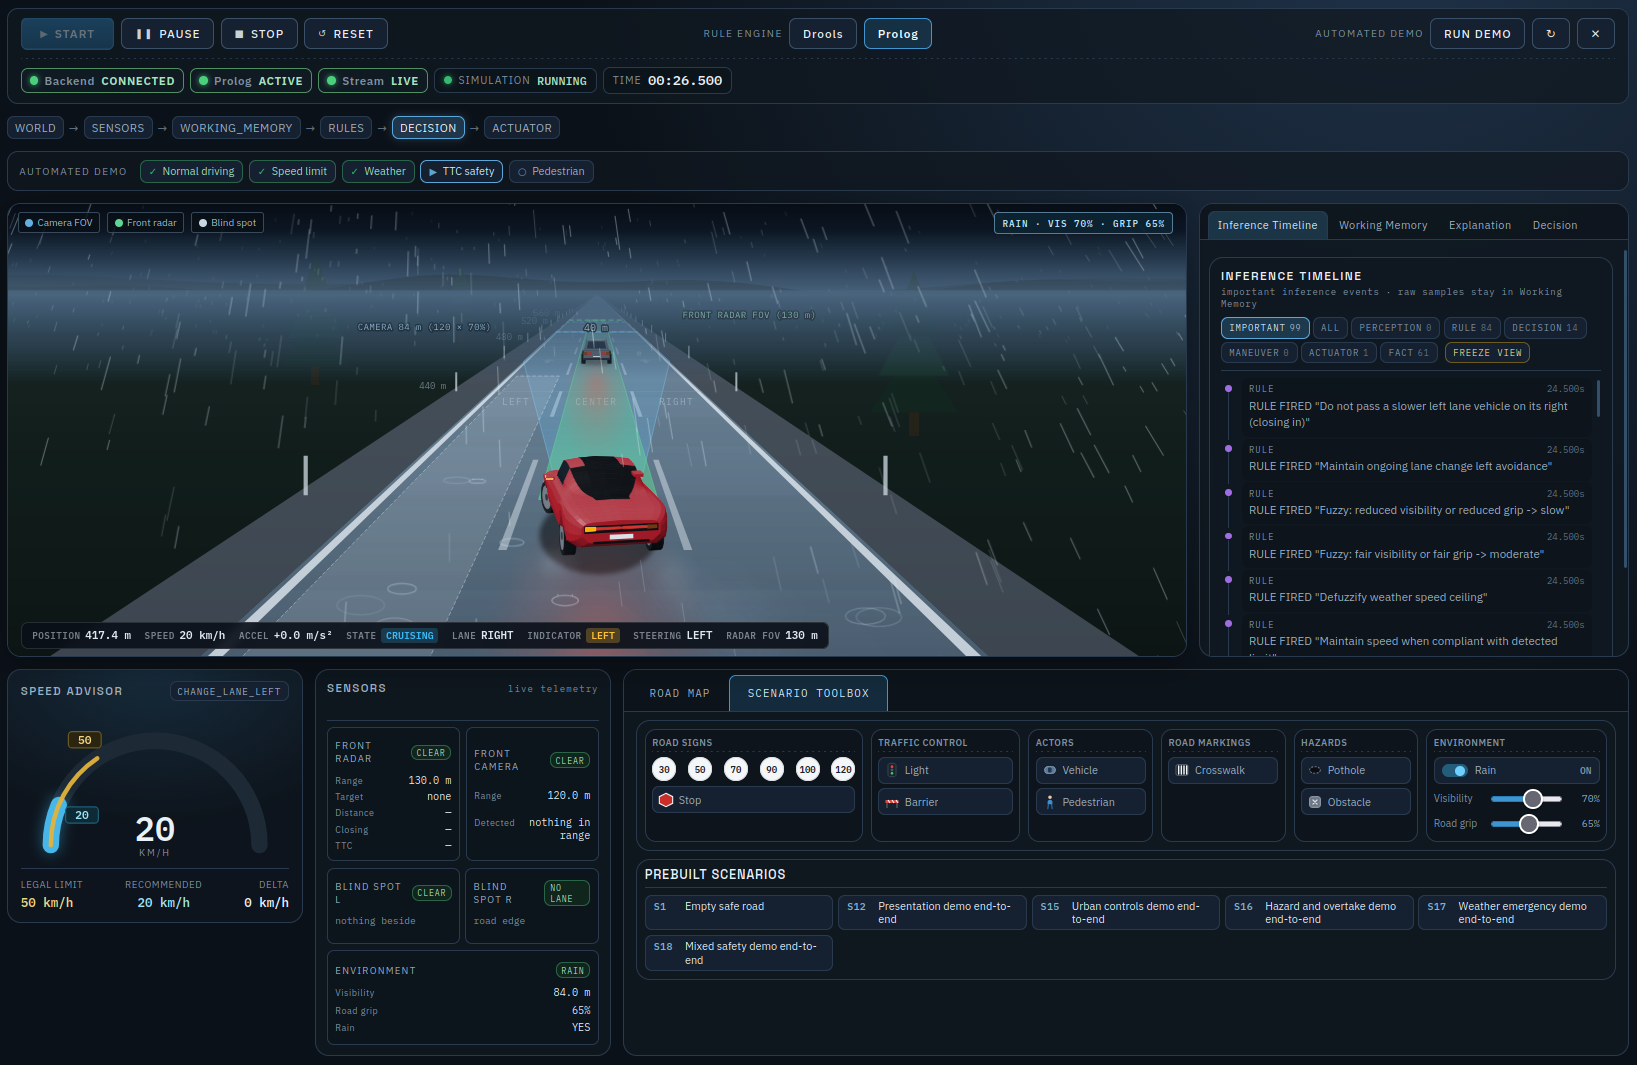
\includegraphics[width=0.72\textwidth]{figuras/screenshot-web-ui.png}
  \caption{Interface Web com o motor Prolog ativo, durante uma ultrapassagem com chuva.}
  \label{fig:interface-web}
\end{figure}

\chapter{Dificuldades e decisões técnicas}
\label{cap:dificuldades}

\section{Correspondência semântica com Drools}
\label{sec:dif-drools}

A dificuldade principal foi reproduzir em Prolog comportamentos que o Drools
oferece diretamente, como memória com estado, eventos com expiração, janelas
temporais, \emph{salience} e reatividade a atualizações. A solução separou o
estado persistente da memória do ciclo, codificou as janelas por
\emph{timestamps} e criou um motor com agenda explícita.

\section{Ordem dos eventos}
\label{sec:dif-eventos}

Eventos relacionados podem chegar em ordens diferentes. O
\cod{driving_state.pl} processa as distâncias frontais antes das restantes
medições para que a velocidade relativa e o TTC atualizem o alvo correto. Este
detalhe evita decisões dependentes da ordem incidental do \emph{array} JSON.

\section{Explicação de condições auxiliares}
\label{sec:dif-auxiliares}

Um \cod{test/1} comum pode ocultar os factos consultados por um predicado
auxiliar. A forma \cod{prove/1} resolve este problema: prova o objetivo por
encadeamento inverso, recolhe os identificadores dos factos lidos e permite
construir uma cadeia explicativa. A mesma decomposição torna possível explicar
por que uma mudança de faixa não é segura.

\section{Conflitos entre velocidade e faixa}
\label{sec:dif-canais}

Uma única ordenação global faria uma proposta de mudança de faixa competir
diretamente com uma travagem, embora controlem dimensões diferentes. O
\cod{DecisionContext} divide as propostas em canal longitudinal e lateral e
aplica depois um veto de segurança. Esta modelação permite travar enquanto se
inicia uma manobra quando isso é seguro, mas bloqueia a manobra perante uma
paragem obrigatória mais importante.

\chapter{Conclusão}
\label{cap:conclusao}

O projeto cumpre o objetivo de integrar Prolog num sistema pericial interativo e
explicável. A contribuição técnica principal é o motor de regras de produção
implementado em \cod{engine.pl}. A agenda determinística, a refração, a
proveniência e o índice de dependências tornam explícitos mecanismos que, noutros
motores, permanecem internos.

A base de conhecimento apresenta dimensão e variedade suficientes para
demonstrar raciocínio reativo, temporal, negativo, difuso e orientado por
objetivos. A integração com Java preserva todas as propostas e separa os canais
de controlo, enquanto a interface permite observar factos, regras e decisões. Os
testes de equivalência com Drools e a execução integral de 598 testes sem falhas
fornecem evidência de correção no contexto do simulador.

A solução deve ser entendida como um protótipo académico de apoio à decisão.
Dentro desse âmbito, oferece uma resposta completa aos critérios de avaliação:
base de conhecimento estruturada, novo motor de inferência, explicações
\emph{How}, \emph{Why} e \emph{Why not}, metaconhecimento, arquitetura
cliente-servidor e demonstração prática.

% As Referências e o Anexo voltam a abrir página.
\quebracapitulotrue

% Todas as entradas de referencias.bib são citadas no texto. O \nocite{*} só
% garante que uma entrada nova, ainda por citar, aparece no fim da lista.
\nocite{*}
\bibliographystyle{unsrt}
\bibliography{referencias}

\appendix
\chapter{Mapeamento entre código e relatório}
\label{anx:mapeamento}

\begin{table}[H]
  \centering
  \caption{Localização no código de cada tema do relatório}
  \label{tab:mapeamento}
  \small
  \begin{tabularx}{\textwidth}{@{}L{5.0cm}V>{\raggedright\arraybackslash}X@{}}
    \toprule
    \textbf{Tema} & \textbf{Localização principal} \\
    \midrule
    \multicolumn{2}{@{}l}{\textit{Motor Prolog (\cref{cap:motor,cap:base-conhecimento,cap:metaconhecimento})}} \\ \linhasep
    Motor de inferência, com meta-conhecimento e suporte para explicações
      & \cod{src/main/prolog/engine.pl} \\ \linhasep
    Estado temporal entre ciclos & \cod{src/main/prolog/driving_state.pl} \\ \linhasep
    Base de conhecimento para apoio à condução autónoma
      & \cod{src/main/prolog/driving_rules.pl} \\ \linhasep
    Interface JSON com o resto do sistema & \cod{src/main/prolog/server.pl} \\ \linhasep
    Regras Drools que a base Prolog replica
      & \cod{src/main/resources/rules/} \\ \linhasep
    \multicolumn{2}{@{}l}{\textit{Integração e arbitragem (\cref{sec:integracao})}} \\ \linhasep
    Integração Java com o processo Prolog & \cod{src/main/java/com/one2drive/projeto1/prolog/} \\ \linhasep
    Contrato comum aos motores
      & \cod{src/main/java/com/one2drive/projeto1/inference/ExpertSystemBackend.java} \\ \linhasep
    Arbitragem, prioridades e constantes enviadas no \cod{reset}
      & \cod{src/main/java/com/one2drive/projeto1/decision/} (\cod{DecisionContext},
        \cod{DecisionPriority}, \cod{StoppingPolicy}) \\ \linhasep
    Cenários da biblioteca & \cod{src/main/resources/scenarios/scenarios.json} \\ \linhasep
    \multicolumn{2}{@{}l}{\textit{Explicações (\cref{cap:explicacao})}} \\ \linhasep
    Registo de cada ciclo e fluxograma de decisão
      & \cod{src/main/java/com/one2drive/projeto1/explanation/},
        \cod{.../history/} \\ \linhasep
    Respostas \emph{How}, \emph{Why} e \emph{Why not} sobre as viagens gravadas
      & \cod{src/main/java/com/one2drive/projeto1/api/service/}
        (\cod{SessionExplanationService}, \cod{AlternativeExplainer}) \\ \linhasep
    Fluxogramas de decisão (a árvore de decisão referida na \cref{sec:base-conteudo})
      & \cod{docs/fluxogramas/} \\ \linhasep
    \multicolumn{2}{@{}l}{\textit{Interface Web (\cref{sec:interface})}} \\ \linhasep
    Aplicação Angular & \cod{frontend/src/app/} \\ \linhasep
    Painéis de explicação e diálogo de perguntas
      & \cod{frontend/src/app/expert-system/} \\ \linhasep
    \multicolumn{2}{@{}l}{\textit{Testes}} \\ \linhasep
    Testes Java (JUnit), raiz & \cod{src/test/java/com/one2drive/projeto1/} \\ \linhasep
    Testes do motor Prolog e de equivalência com o Drools
      & \cod{src/test/java/com/one2drive/projeto1/prolog/} \\ \linhasep
    Testes de simulação (E2E) e \emph{benchmark} do índice
      & \cod{src/test/java/com/one2drive/projeto1/simulation/}
        (\cod{DependencyIndexBenchmarkTest}) \\ \linhasep
    Testes Playwright da interface Web & \cod{frontend/e2e/} (\cod{frontend/playwright.config.ts}) \\
    \bottomrule
  \end{tabularx}
\end{table}


\end{document}
